\documentclass{article}
\usepackage{graphicx} % Required for inserting images
\usepackage{amsmath}
\title{CSC376 - ASSIGNMENT 3}
\author{Jott Girn and Stephen Le}
\date{November 2024}

\begin{document}
 \maketitle 
 \begin{center}
     Resources used: Lecture slides, and the Modern Robotics textbook.
     
 \end{center}
 \textbf{Question 1}:\\

Starting with $p_z$, by looking at the diagram provided for this assignment, we can see that:
$$p_z = L + (\sqrt(2)L+\theta_2)cos(\pi/4) + L = 3L + \frac{\theta_2}{\sqrt(2)}$$
Solving for $\theta_2$:
$$\theta_2 = \sqrt(2)(p_z - 3L)$$
Thus we have $$\frac{\theta_2}{\sqrt{2}} = p_z - 3L $$ 
In addition, given that $0<=\theta_2<=\sqrt{2}L$, we can see that $3L<=p_z<=4L$.
\\
\\
Now, for the solutions to $\theta_3$ and $\theta_1$, we must analyze a number of different cases based on the values of $p_x$, $p_y$ and $p_z$. If a given $p_x$, $p_y$ and $p_z$ does not fit one of these cases, there is no solution for it[it is impossible to move the robot there].
\newpage
\textbf{Case 1}: $0 < p_z - 3L < \sqrt{p_x^2 + p_y^2} < p_z - L < 3L$
\\
\\
\begin{center}
            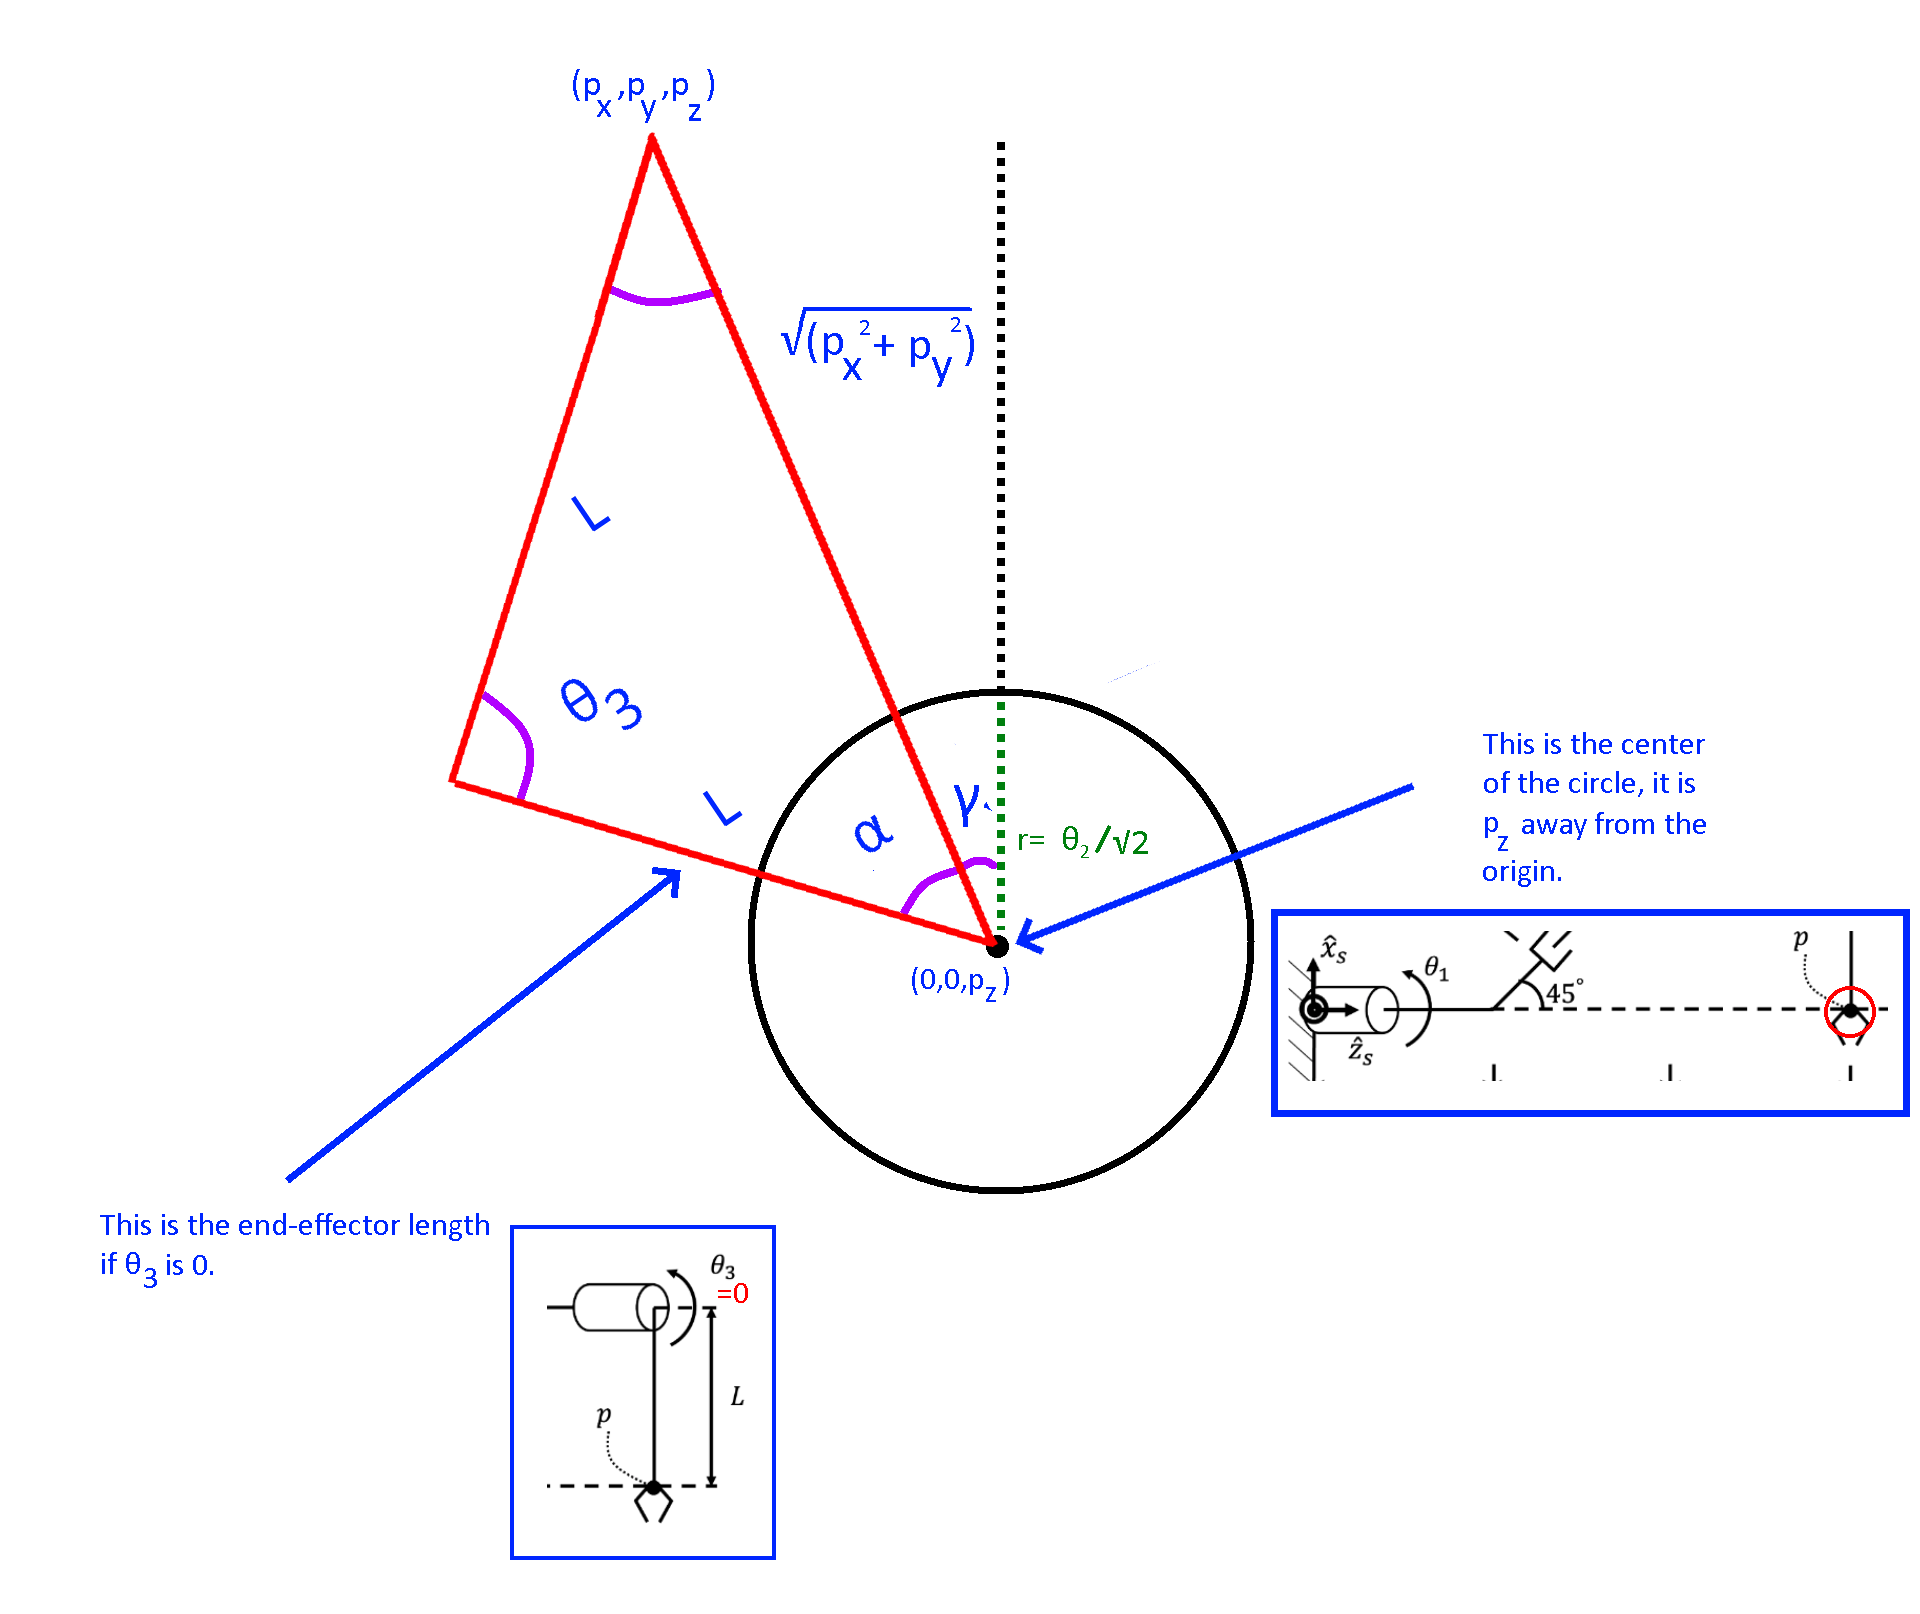
\includegraphics[scale=0.3]{diagram_q1.png}
            Figure 1: Diagram to find $\theta_3$ and $\theta_1$ in Case 1
 \end{center}
Using the cosine law based on what is seen in Figure 1, we can derive:
$$p_x^2 + p_y^2 = (p_z -2L)^2 + L^2 - 2(L)(p_z-2L)cos(\theta_3)$$
Rearranging this to solve for $\theta_3$:
$$\theta_3 = cos^{-1}(\frac{(p_z -2L)^2 + L^2}{2(L)(p_z-2L)cos(\theta_3)}) $$
\\
\\
This is the only solution for $\theta_3$ in this case due to the joint limits of $\theta_3$ being $[0, \pi]$. 
\\
\\
Next, with Figure 1, we define $\Gamma$ as the following:
$$\Gamma = atan2(p_y,p_x)$$
Looking at $L^2$ with the cosine law we can finally solve:
$$L^2 = (L+\frac{\theta_2}{\sqrt{2}})^2 + p_y^2 + p_x^2 -2(L+ \frac{\theta_2}{\sqrt{2}})(\sqrt{p_x^2 + p_y^2})cos(\alpha)$$
Using inverse cosine, we can solve for $\alpha$:
$$\alpha = cos^{-1}[\frac{(L+\frac{\theta_2}{\sqrt{2}})^2 + p_y^2 + p_x^2}{2(L+ \frac{\theta_2}{\sqrt{2}})(\sqrt{p_x^2 + p_y^2})}]$$
Plugging in the equation solved at the start where $\theta_2/\sqrt{2} = p_z-3L$:
$$\alpha = cos^{-1}[\frac{(p_z-2L)^2 + p_y^2 + p_x^2}{2(p_z-2L)(\sqrt{p_x^2 + p_y^2})}]$$
Given the restrictions on $\theta_3$ and looking at Figure 1, we can see that the only solution for $\theta_1$ in this case is:
$$\theta_1 = \Gamma + \alpha$$
\\
\\
\textbf{Case 2}: $ 2L <= p_z - L = \sqrt{p_x^2 + p_y^2} <= 3L$
\\
\\
 \begin{center}
            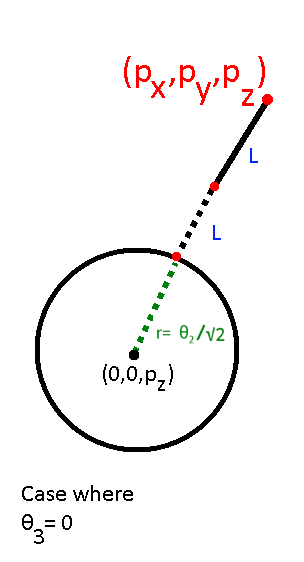
\includegraphics[scale=0.5]{a3robot1.png}\\
            Figure 2: Diagram to find $\theta_3$ and $\theta_1$ in Case 2
            \\
 \end{center}
We can see from Figure 2 that in this case, $\theta_{3} = 0$ must be true, and $\theta_1 = atan2(p_y,p_x)$. 
\\
\\
\textbf{Case 3}: $0 < p_z - 3L = \sqrt{p_x^2 + p_y^2} <= L $
\\
\\
 \begin{center}
            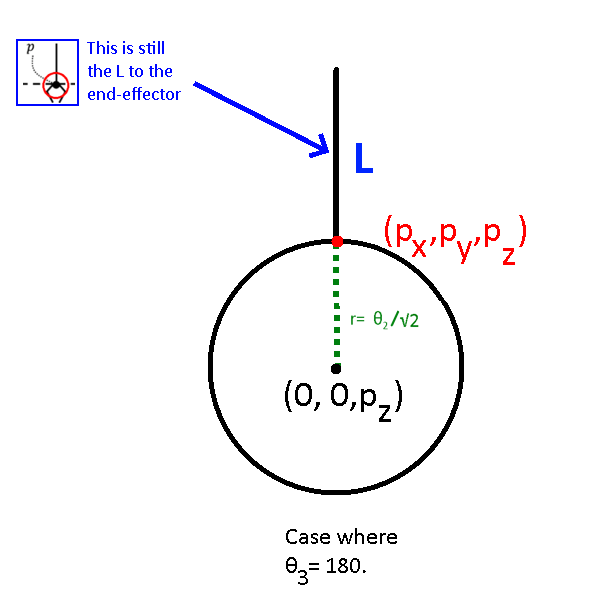
\includegraphics[scale=0.5]{a3robot2_fix.png}\\
            Figure 3: Diagram to find $\theta_3$ and $\theta_1$ in Case 3
            \\
 \end{center}
We can see from Figure 3 that in this case, $\theta_{3} = \pi$ must be true, and $\theta_1 = atan2(p_y,p_x)$. 
\\
\\
\textbf{Case 4}: $p_x = 0, p_y = 0, p_z = 3L$
\\
\\
This is p when the robot is in its zero position. We can easily see from the diagram provided for this assignment that $\theta_3=0$ and $\theta_2=0$ must both be true. Finally, given that p in this case is on the same axis of rotation as $\theta_1$, there are infinite solutions to $\theta_1$ for this position. 
\\
\\
\textbf{Question 2}:
All the comments are in the code itself.\\
\textbf{Question 3}:
\textbf{ Part a }:\\
For each of the graphs:
\begin{itemize}
    \item A: Fifth-order acceleration
\item B: Third order velocity
\item C: Trapezoid acceleration
\item D: Trapezoid velocity
\item E: Third-order acceleration 
\item F: fifth order velocity
\end{itemize}
Discussing the advantages and disadvantages of each in comparison:
\begin{itemize}
    \item Fifth order:
    \begin{itemize}
        \item Advantage: Motion is smoother b/c acceleration at the beginning and end are constrained to 0, resulting in smoother motion, no vibrations, it is much smoother then the third-order polynomial.
        \item  Disadvantage:  More complex than trapezoidal, does not accelerate as fast
    \end{itemize}
    \item Trapezoid:
      \begin{itemize}
        \item Advantage:Reaches max straight line motion velocity the fastest, it has the largest v and a satifsying the equations over the limit.
        \item  Disadvantage:  It is not as smooth as cubic or fifth order, it is much more "snappy"
    \end{itemize}
    \item Third order:
    \begin{itemize}
        \item Advantage: Simpler than quintic, smoother than trapezoidal
        \item  Disadvantage:  Not as fast a trapezoidal, the acceleration jumps at the start at the end, compared to the trapezoidal and fifth-order accelerations, the acceleration jumps discontinuously at the start and end of the time.
    \end{itemize}
\end{itemize}
\textbf{ Part b }:\\
From the description of the problem, we can see that:
\begin{align}
    \theta_{end} &= 300\\
    \theta_{start} &= 50\\
    \dot{\theta}_{limit} &= 25\\
    \ddot{\theta}_{limit} &= 50\\
\end{align}
We wish to solve for maximum velocity, recall that from the lectures, it is known that we can solve for the largest $v$ and $a$, in the fastest straight line possible[minimum time]:
\begin{align}
    |\theta_{end}-\theta_{start}v| & \leq  \dot{\theta}_{limit}\\ 
     |\theta_{end}-\theta_{start}a| & \leq  \ddot{\theta}_{limit}\\
\end{align}
Plugging in the values we have gotten and solving:
\begin{align}
    |(300-50)v| & \leq  25\\ 
    |250v| & \leq 25\\
    |v|  &\leq 25/250\\
    |v|  &\leq 0.1\\
     |(300-50)a| & \leq  50\\
     |250a| & \leq 50\\
     |a| & \leq 50/250\\
     |a|  &\leq 0.2
\end{align}
Setting the acceleration and velocity to the max, now have the maximum acceleration and velocity known to solve, now, from lectures, it is known that a "bang-bang" motion is reached if $v^2/a > 1$, fortunately, $v^2/a = 0.1^2/0.2-0.05$, therefore, we have a normal trapezoidal motion. In chapter 9.2, page 334 of the modern robotics textbook, it was shown that for any $v^2/a\leq 1$, the following yields the minimum time $T$:
$$T= \frac{a+v^2}{va}$$
Plugging in the values, we finally obtain:
$$T=\frac{0.2+0.1^2}{0.2 \times 0.1}=10.5$$
Therefore, the minimum time is 10.5.
\end{document}
